\documentclass{article}

% Target journal: Molecular Phylogenetics and Evolution
%
% From author guidelines:
%
% Short communications of approximately 3000 words are also accepted. 
% These papers should contain no more than two figures, two tables, and thirty references. 
% A short abstract of fewer than 200 words is acceptable.


% Annotation/feedback commands
\newcommand*\rampal[1]{\textcolor{red}{\textbf{[RSE: #1]}}}
\newcommand*\richel[1]{\textcolor{orange}{\textbf{[RJCB: #1]}}}
\newcommand*\gio[1]{\textcolor{green}{\textbf{[GL: #1]}}}

% Bibliography
\usepackage{natbib}
\bibpunct{(}{)}{;}{a}{}{;}

\usepackage[english]{babel}

% Use 'It was found that something is something (Name 1234)' style
\setcitestyle{authoryear,open={},close={}}

% Affiliations
\usepackage{authblk}
\title{The error in Bayesian phylogenetic reconstruction when speciation co-occurs}

\author[1]{Giovanni Laudanno}
\author[1]{Rich\`el J.C. Bilderbeek}
\author[1]{Rampal S. Etienne}
\affil[1]{Groningen Institute for Evolutionary Life Sciences, University of Groningen, Groningen, The Netherlands}

% Use double spacing
\usepackage{setspace}
\doublespacing

\usepackage{pgf}
\usepackage{hyperref}
\usepackage{verbatim}
  
% Adds numbered lines
\usepackage{lineno}
\linenumbers

\hyphenation{
  BEAST
  Pa-ra-me-ter
  Drum-mond 
  Bayes-ian 
  Mr-Bayes 
  ap-proach-es 
  Rev-Bayes 
  cre-ate
  spe-ci-a-tion-com-ple-tion
  pro-trac-ted
 }

\begin{document}

\maketitle

%%%%%%%%%%%%%%%%%%%%%%%%%%%%%%%%%%%%%%%%%%%%%%%%%%%%%%%%%%%%%%%%%%%%%%%%%%%%%%%%%%%%%%
\begin{abstract}

  % From 'How to construct a Nature summary paragraph'

  % A short abstract of fewer than 200 words is acceptable.

  % One or two sentences providing a basic
  % introduction to the field,
  % comprehensible to a scientist in any discipline.
  

  % Two to three sentences of
  % more detailed background, comprehensible to
  % scientists in related disciplines.
  

  % One sentence clearly stating the general
  % problem being addressed by this particular
  % study.
  

  % One sentence summarising the main
  % result (with the words “here we show”
  % their equivalent).
  

  % Two or three sentences explaining what
  % the main result reveals in direct
  % comparison to what was thought to be the case
  % previously, or how the main result adds to
  % previous knowledge.

  % One or two sentences to put the results into a
  % more general context.


  % Two or three sentences to provide a
  % broader perspective, readily comprehensible
  % to a scientist in any discipline, may be included
  % in the first paragraph if the editor considers that the accessibility of the paper is significantly enhanced
  % by their inclusion. Under these circumstances, the length of the paragraph can be up to 300 words.
  % (The above example is 190 words without the final section, and 250 words with it).



\end{abstract}

{\bf Keywords:} computational biology, evolution, phylogenetics, Bayesian analysis, tree prior
%%%%%%%%%%%%%%%%%%%%%%%%%%%%%%%%%%%%%%%%%%%%%%%%%%%%%%%%%%%%%%%%%%%%%%%%%%%%%%%%%%%%%%
\gio{@richel: A) I am throwing down some main points to follow to develop a convincing story that follows a clear logic. It might happen that some of these points are repeated and/or in the wrong order. We need to check that.}
\gio{@richel: B) According to my fine graining approach we should at each step deepen every small section. At a certain level I think we can start to re-coarse-grain what we wrote to create the abstract.}

%%%%%%%%%%%%%%%%%%%%%%%%%%%%%%%%%%%%%%%%%%%%%%%%%%%%%%%%%%%%%%%%%%%%%%%%%%%%%%%%%%%%%%
\section{Introduction}
\begin{itemize}

\item Tools like BEAST provide the possibility to infer a phylogeny from genetic data (DNA, RNA, proteins).

\item There are a number of options that can be set up while using BEAST.

\item Current limits in current tools.

\item BEAST2 gives us the possibility to introduce new tree priors to infer phylogenies based on different assumptions.

\item One of these is the multiple birth hypothesis.

\item Multiple birth hypothesis can be useful to explain a phenomenon that have always puzzled evolutionary biologists: what are the drivers of the diversification processes for those phylogenies that show an impressive amount of speciation events in relatively short times.
The (constant-rate) birth-death (BD) model embodies the common assumption that 
only a single speciation event can occur at any given time.
The MBD model relaxes this assumption, allowing events in which 
large-scale environmental changes lead to a great number of species 
in relatively short time intervals. Such hypothesis can be useful to describe, for example, 
systems like cichlid fish diversification in the 
African Great Lakes: Malawi, Tanganyika and Victoria (\cite{janzen2016}, \cite{janzen2017}).

\item However it can be argued that current tree priors could be good enough to detect such events involving, at the same time, a lower level of complexity. If this is the case one should always be more keen to adopt the simplest model.

\item Here we present our study with the aim of proving that there is indeed the necessity of a new tree prior for such cases.

\end{itemize}
%%%%%%%%%%%%%%%%%%%%%%%%%%%%%%%%%%%%%%%%%%%%%%%%%%%%%%%%%%%%%%%%%%%%%%%%%%%%%%%%%%%%%%

%%%%%%%%%%%%%%%%%%%%%%%%%%%%%%%%%%%%%%%%%%%%%%%%%%%%%%%%%%%%%%%%%%%%%%%%%%%%%%%%%%%%%%
\section{Methods}

\subsection{Model}
\begin{itemize}

\item Current phylogenetic tools assume that only a single speciation event can occur at any given time.
While this assumption is useful to construct a wide variety of successful 
models (for example: \cite{Maddison2007biSSE}, \cite{Valente2015}, \cite{etienne2012diversity}, \cite{etienne2014estimating}),
they disallow for environmental changes that trigger speciations in multiple clades at a same point in time.

\item The (constant-rate) birth-death (BD) model embodies the common assumption that 
only a single speciation event can occur at any given time.
The MBD model relaxes this assumption, allowing events in which 
large-scale environmental changes lead to a great number of species 
in relatively short time intervals. Such hypothesis can be useful to describe, for example, 
systems like cichlid fish diversification in the 
African Great Lakes: Malawi, Tanganyika and Victoria (\cite{janzen2016}, \cite{janzen2017}).

\item In the MBD model, parameters $\lambda$ and $\mu$ correspond, respectively, 
to the usual per-species speciation and extinction rates. 
Additionally, $\nu$ is the rate at which an environmental change is triggered.
When such event is triggered, all species present in the phylogeny at that moment
have a probability $q$ to speciate (independent on $\lambda$).
The number of species that speciate due to this can also be zero. 

\item It is also possible to write down a likelihood function for such processes as in \cite{mbd}.
    
\end{itemize}

\subsection{Simulations}
\begin{itemize}

\item To prove our hypothesis we simulate two twin datasets. All the simulations are produced in continuous time, using the Doob-Gillespie algorithm. 

\item We start simulating a number (100?) of trees for the MBD model. We then use, for each tree, the 'pirouette' package (\cite{pirouette}) to obtain the sequence alignments corresponding to the given tree. 'pirouette' then calls BEAST to use these alignments to infer a posterior distribution of phylogenies. To perform this operation BEAST will use a BD prior.

\item For each tree 
\gio{QUESTION 1: Do we convert each single tree or the entire distribution?} 
\richel{SUGGEST 1: Each tree, as (1) it's easier (2) I so no benefit (nor difference) with the second option} 
generated under the MBD model we aim to generate a "twin" tree under the BD model in order to perform the same analysis and compare the results. To do so we need to be sure that the comparison is fair. The method we adopt to achieve this goal is to impose that the average number of substitution will be the same 
\gio{QUESTION 2: What criterion are we going to use? Same amount of information? Same number of tips? Something else? The answer has to be given mostly according to biological reasons, I think.}.
\richel{SUGGEST 2: I would prefer the same amount of tips and mutations. See figure.}
\item Here we explain how the conversion is done, with formulas if necessary.

\begin{figure}[!htbp]
  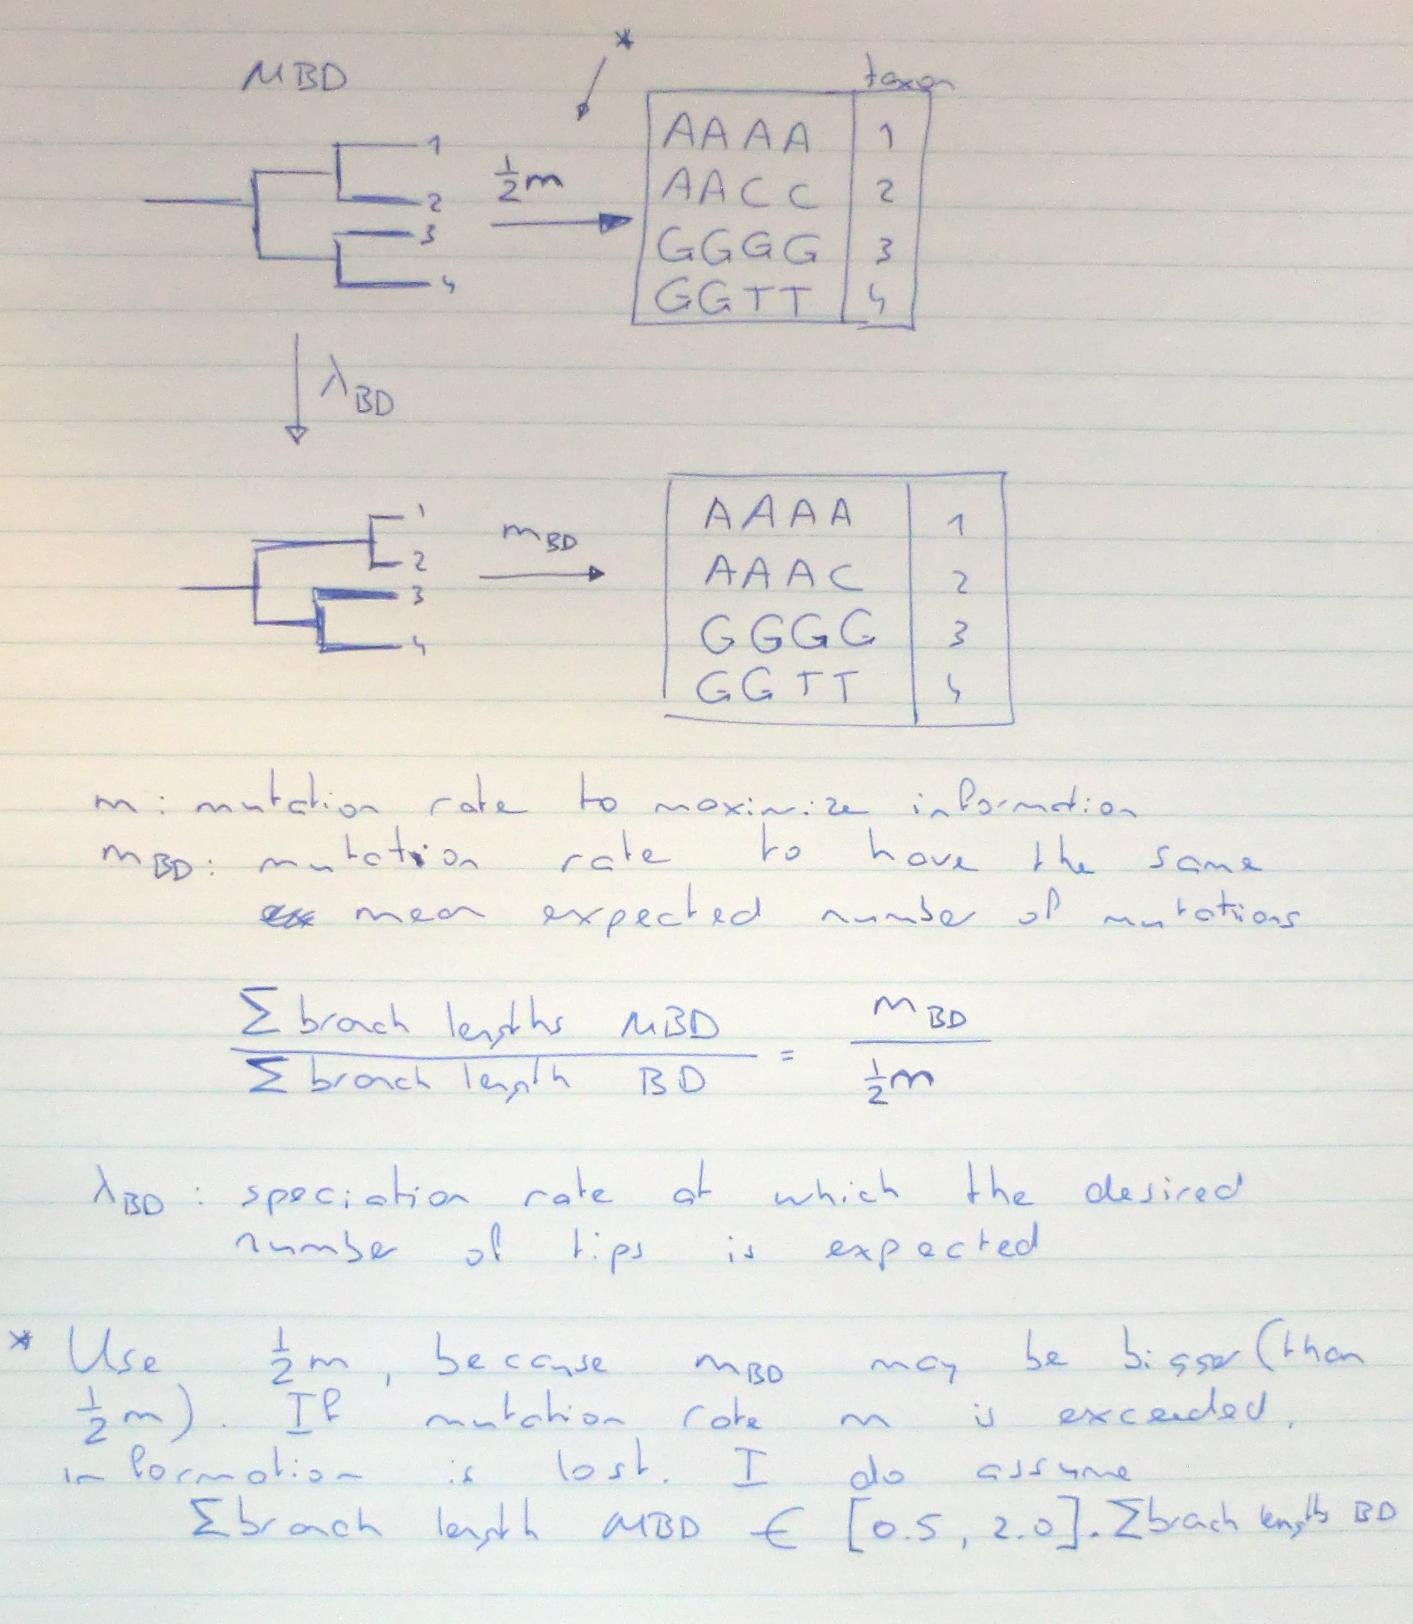
\includegraphics[width=\textwidth]{mbd.jpg}
  \caption{
    How to create twin trees and alignments. From a focal MBD tree, a twin tree is produced as 
    such: (1) estimate the $\lambda_{BD}$ to get the same expected number of tips, (2) simulate a BD tree with that amount of tips (discard trees with different number of tips), (3) estimate a mutation rate to get an alignment with the same expected number of mutations, (4) simulate alignments with that amount of mutations (discard those that don't, the picture shows an alignment that should be discarded) 
  }
\end{figure}

\item We explained how we set the parameters for each twin BD tree. Using this rules we generate a BD dateset. We repeat the raket analysis, producing alignments for each tree and subsequently using BEAST to produce a posterior for each of them.

\item Now we have to datasets of posteriors to compare, one for the BD model and one for the MBD model.

\item To compare the results for the two models we measure the inference error using the nLTT statistic between known/true tree and posterior/inferred trees.
\richel{Rewrote this a bit. I suggest to drop the Bayes factor for now. It can be used if we would let BEAST2 infer with different nucleotide substitution models (a.k.a. site models), to answer the question: which nucleotide substitution model should be used in inference? Using different site models was Rampal's idea and I hope we can cite the raket paper to demonstrate it does not matter}

\item The BF method allows us to compare the two marginal distributions. \gio{insert mathematical formula}

\end{itemize}
%%%%%%%%%%%%%%%%%%%%%%%%%%%%%%%%%%%%%%%%%%%%%%%%%%%%%%%%%%%%%%%%%%%%%%%%%%%%%%%%%%%%%%

%%%%%%%%%%%%%%%%%%%%%%%%%%%%%%%%%%%%%%%%%%%%%%%%%%%%%%%%%%%%%%%%%%%%%%%%%%%%%%%%%%%%%%
\section{Results}
\begin{itemize}

\item

\item

\end{itemize}
%%%%%%%%%%%%%%%%%%%%%%%%%%%%%%%%%%%%%%%%%%%%%%%%%%%%%%%%%%%%%%%%%%%%%%%%%%%%%%%%%%%%%%

%%%%%%%%%%%%%%%%%%%%%%%%%%%%%%%%%%%%%%%%%%%%%%%%%%%%%%%%%%%%%%%%%%%%%%%%%%%%%%%%%%%%%%
% Bibliography % MEE style
\bibliographystyle{mee}
\bibliography{article}
%%%%%%%%%%%%%%%%%%%%%%%%%%%%%%%%%%%%%%%%%%%%%%%%%%%%%%%%%%%%%%%%%%%%%%%%%%%%%%%%%%%%%%

%%%%%%%%%%%%%%%%%%%%%%%%%%%%%%%%%%%%%%%%%%%%%%%%%%%%%%%%%%%%%%%%%%%%%%%%%%%%%%%%%%%%%%
\appendix


%%%%%%%%%%%%%%%%%%%%%%%%%%%%%%%%%%%%%%%%%%%%%%%%%%%%%%%%%%%%%%%%%%%%%%%%%%%%%%%%%%%%%%


\end{document}